\documentclass{article}\usepackage[]{graphicx}\usepackage[]{color}
%% maxwidth is the original width if it is less than linewidth
%% otherwise use linewidth (to make sure the graphics do not exceed the margin)
\makeatletter
\def\maxwidth{ %
  \ifdim\Gin@nat@width>\linewidth
    \linewidth
  \else
    \Gin@nat@width
  \fi
}
\makeatother

\definecolor{fgcolor}{rgb}{0.345, 0.345, 0.345}
\newcommand{\hlnum}[1]{\textcolor[rgb]{0.686,0.059,0.569}{#1}}%
\newcommand{\hlstr}[1]{\textcolor[rgb]{0.192,0.494,0.8}{#1}}%
\newcommand{\hlcom}[1]{\textcolor[rgb]{0.678,0.584,0.686}{\textit{#1}}}%
\newcommand{\hlopt}[1]{\textcolor[rgb]{0,0,0}{#1}}%
\newcommand{\hlstd}[1]{\textcolor[rgb]{0.345,0.345,0.345}{#1}}%
\newcommand{\hlkwa}[1]{\textcolor[rgb]{0.161,0.373,0.58}{\textbf{#1}}}%
\newcommand{\hlkwb}[1]{\textcolor[rgb]{0.69,0.353,0.396}{#1}}%
\newcommand{\hlkwc}[1]{\textcolor[rgb]{0.333,0.667,0.333}{#1}}%
\newcommand{\hlkwd}[1]{\textcolor[rgb]{0.737,0.353,0.396}{\textbf{#1}}}%
\let\hlipl\hlkwb

\usepackage{framed}
\makeatletter
\newenvironment{kframe}{%
 \def\at@end@of@kframe{}%
 \ifinner\ifhmode%
  \def\at@end@of@kframe{\end{minipage}}%
  \begin{minipage}{\columnwidth}%
 \fi\fi%
 \def\FrameCommand##1{\hskip\@totalleftmargin \hskip-\fboxsep
 \colorbox{shadecolor}{##1}\hskip-\fboxsep
     % There is no \\@totalrightmargin, so:
     \hskip-\linewidth \hskip-\@totalleftmargin \hskip\columnwidth}%
 \MakeFramed {\advance\hsize-\width
   \@totalleftmargin\z@ \linewidth\hsize
   \@setminipage}}%
 {\par\unskip\endMakeFramed%
 \at@end@of@kframe}
\makeatother

\definecolor{shadecolor}{rgb}{.97, .97, .97}
\definecolor{messagecolor}{rgb}{0, 0, 0}
\definecolor{warningcolor}{rgb}{1, 0, 1}
\definecolor{errorcolor}{rgb}{1, 0, 0}
\newenvironment{knitrout}{}{} % an empty environment to be redefined in TeX

\usepackage{alltt}
\usepackage{amssymb}
\usepackage{enumerate}
\usepackage{relsize}
\usepackage{url} % not crucial - just used below for the URL
\usepackage{multirow}
\usepackage{multicol}
\usepackage{rotating}
\usepackage{relsize}
\usepackage{bm}
\usepackage{framed}
%\usepackage{empheq}
\usepackage{hyperref}
\usepackage{multicol}
\usepackage{setspace}
\usepackage{enumerate}
\usepackage{footnote}
\usepackage{authblk}
\usepackage{float}
\usepackage{longtable}
\def\a{\alpha}      \def\b{\beta}     \def\g{\gamma}   \def\d{\delta}
\def\th{\theta}     \def\lm{\lambda}  \def\sg{\sigma}
\def\lmone{\lambda_{1n}}
 \def\lmtwo{\lambda_{2n}}
\def\bzero{{\mathbf 0}}  \def\bone{{\mathbf 1}} \def\btwo{{\mathbf 2}}
\def\bW{{\mathbf W}}
\def\bB{{\mathbf B}}
\def\bA{{\mathbf A}} \def\bC{{\mathbf C}} \def\bD{{\mathbf D}} \def\bE{{\mathbf E}}
\def\bF{{\mathbf F}} \def\bS{{\mathbf S}} \def\bT{{\mathbf T}}
\def\bG{{\mathbf G}} \def\bH{{\mathbf H}} \def\bK{{\mathbf K}} \def\bI{{\mathbf I}}
\def\bL{{\mathbf L}} \def\bN{{\mathbf N}} \def\bP{{\mathbf P}} \def\bQ{{\mathbf Q}}
\def\bR{{\mathbf R}} \def\bS{{\mathbf S}} \def\bT{{\mathbf T}} \def\bU{{\mathbf U}}
\def\bV{{\mathbf V}} \def\bW{{\mathbf W}} \def\bX{{\mathbf X}} \def\bY{{\mathbf Y}}
\def\bZ{{\mathbf Z}}
\def\bM{\boldsymbol M}
\def\bPi{{\mathbf \Pi}}

\def\tbM{\widetilde{\boldsymbol M}}
\def\tT{\widetilde{T}}

\def\ba{{\mathbf a}} \def\bb{{\mathbf \beta}}
\def\bd{{\mathbf d}} \def\be{{\mathbf e}}
\def\bdf{{\mathbf f}} \def\bg{{\mathbf g}} \def\bh{{\mathbf h}}

\def\bell{{\mathbf l}} \def\bp{{\mathbf p}} \def\bq{{\mathbf q}}
\def\br{{\mathbf r}} \def\bs{{\mathbf s}} \def\bt{{\mathbf t}}
\def\bu{{\mathbf u}} \def\bv{{\mathbf v}} \def\bw{{\mathbf w}}
\def\bx{{\mathbf x}} \def\by{{\mathbf y}} \def\bz{{\mathbf z}}
\def\bSigma{{\mathbf \Sigma}}
%\newcommand{\bm}{\mathbf}
\newcommand{\argmin}[2]{\underset{#1}{\arg\min} \{ #2\}}
\newcommand{\Argmin}[2]{\underset{#1}{\arg\min} \Bigg \{ #2 \Bigg \} }
\newcommand{\RR}{\mathbb{R}}

%% new
 \def\bbeta{{\mathbf \beta}}
 \def \tbbeta{{ \tilde{\mathbf \beta}}}
 \def \tbw{{\tilde{\bw}}}
 \def \cR{{\cal {R}}}
 \def \hbw{{\hat{\bw}}}
 \def \hbbeta{\mathbf {\hat{\beta}} }
 \def \hbeta{\hat{\b}}
 \def \hw{{\hat{w}}}
 \def \hb{{\hat{\b}}}
 \def \eps{ \epsilon}
 \def \btheta{\mathbf \theta}
 \def \bPsi{\mathbf \Psi }
 \def \bOmega { \mathbf \omega}
 \def \veps{\epsilon}
 \def \bveps{ \mathbf \epsilon}
 \def \cA{ \mathbb{A}} % dont know what it is \mathbb{text}
 \def \beps {\mathbf \epsilon }
\def \tbnu{ \tilde{\mathbf{\nu}}}
\def \tnu { \tilde{\nu}}
\def \hbtheta { \hat{\mathbf \theta}}
\def \bpsi {\mathbf \psi }
\def \bTheta { \mathbf \Theta}
\def \rm { }
\def \tbW { \tilde{\mathbf W}}
\def \bnu { \mathbf \nu}
\def \hbSigma {  \hat{ \mathbf \Sigma}}
\def \diag {diag}
\IfFileExists{upquote.sty}{\usepackage{upquote}}{}
\begin{document}
\section{Numerical Result}



% ----------------------------- Variable Selection for Low dimensional case ------------------------------------%
\begin{table}[thp]
	\begin{center}
	 \caption{Variable Selection Results for Example 1 ($\bbeta=(3,2,1.5,0,0,0,0,0)'$ with 10\% outliers ) }\label{table-selection-low1}
	\begin{tabular}{ccccccccccc}\\\hline\hline
	    Method  & CFR (\%) & OFR (\%) & AN & TIME & & & CFR (\%) & OFR (\%) & AN & TIME\\ \hline
	
	   & \multicolumn{4}{c} {\bf Case A} & && \multicolumn{4}{c} {\bf Case B}  \\
	   
	    ALasso & 74 & 23 & 3.29  & 0.8
	         &&& 63 & 25 & 3.25 & 0.78\\
	    
	    sLTS & 9 & 89 & 6.19  &  358.85
	         &&& 14 & 86 & 5.92 &  357.24\\
	    
	    MMNNG & 68 & 25 & 3.25  &  691.33
	    &&& 88 & 12 & 3.13 &  682.07\\
	    
	    SROS & 21 & 76 & 4.31 &  56.67 & && 31 & 69 & 4.24 & 51.79 \\
	         
	    %PAWLS(0) & 58 & 41 & 3.51  &  && 61 & 39 & 3.48 \\
	    SROS-2 & 46 & 53 & 3.66 &  13.49 &&& 67 & 33 & 3.38 &  13.09\\
	    ASROS-2 & 71 & 24 & 3.24 &  13.66 &&& 87 & 13 & 3.14 &  13.81\\
	    
	    PAWLS & 38 & 56 & 3.68 &  16.41 &&& 64 & 36 & 3.42 &  19.32\\
	    APAWLS & 61 & 28 & 3.27 &  20.04 &&& 89 & 11 & 3.11 &  20.18\\
	\\
	   & \multicolumn{4}{c} {\bf Case C} & &  & \multicolumn{4}{c} {\bf Case D}\\
	   
	    ALasso & 3 & 2 & 1.94 & 0.73 &  && 0 & 19 & 2.52 & 0.99\\
	    
	    sLTS & 28 & 72 & 5.34  &  384.69& && 21 & 79 & 5.71 &  398.44\\
	    
	    MMNNG & 72 & 12 & 2.95  &  673.93 &&& 63 & 16 & 3.25  &  682.47\\
	    
	    SROS & 41 & 50 & 3.7  &  50.24 & && 8 & 80 & 4.76  &  50.31\\
	    %PAWLS(0) & 56 & 43 & 3.59 & && 44 & 52 & 4.13 \\
	    SROS-2 & 45 & 53 & 3.76  &  13.44& && 61 & 32 & 3.91 &  15.04\\
	    ASROS-2 & 78 & 17 & 3.18  &  14.06& && 70 & 17 & 3.42 &  15.74\\
	    
	     PAWLS & 52 & 44 & 3.64  &  21.1& && 98 & 0 & 2.98 &  22.83\\
	    APAWLS & 74 & 20 & 3.19  &  21.78& && 97 & 0 & 2.97 &  23.66\\
	    \\
	    
	     & \multicolumn{4}{c} {\bf Case E} & &  \\
	     ALasso & 5 & 10 & 2.72 & 0.72 &  &\\
	    
	    sLTS & 23 & 77 & 5.7  &  383.1& &\\
	    
	    MMNNG & 73 & 10 & 3.04  &  675.46 &&\\
	    
	     SROS & 26 & 61 & 4.45  &  50.08 & &\\
	    %PAWLS(0) & 56 & 55 & 5.59 & && 55 & 52 & 5.15 \\
	     SROS-2 & 29 & 40 & 3.91  &  13.78& &\\
	    ASROS-2 & 48 & 14 & 3.26  &  14.51& &\\
	    
	    PAWLS & 55 & 39 & 3.48  &  21.01& &\\
	    APAWLS & 79 & 15 & 3.16  &  22.5& &\\
	    
	        \hline \hline
	\end{tabular}
	\end{center}
	\end{table}
	
	%------------------------------------ Low dimensional case (combined) ------------------------------%
		\begin{table}[thp]
	\begin{center}
	 \caption{Variable Selection and outliers detection Results for Example 1 ($\bbeta=(3,2,1.5,0,0,0,0,0)'$ with 10\% outliers )}\label{table1}
	\begin{tabular}{ccrrrrrrrrrrrr}\\\hline\hline
	  & & \multicolumn{5}{c} {Variable Selection} &&  \multicolumn{5}{c} {Outliers detection} & \\
	   Case & Method & CFR & OFR  & AN & FP& FN  &  M & S  & JD & FP & FN  & TIME\\ \hline
	  \multirow{8}{*}{{\bf A}}
	      & ALasso & 74 & 23 & 3.29 & 
	      99 & 7.5 & - & - & - & - & - & 0.8\\
	
	      & MMNNG & 68 & 25 & 3.25 & 
	      97 & 8.2 & - & - & - & - & - & 691.33\\
	      
	      & SROS & 21 & 76 & 4.31 & 
	      99 & 27.6 & - & - & - & - & - & 56.67\\
	      
	      & SROS-2 & 46 & 53 & 3.66 & 
	      99.7 & 15.4 &
	      0 & 0.02 & 1
	      & \ensuremath{NaN} & 0.01 & 13.49\\
	      
	     & ASROS-2 & 71 & 24 & 3.24 & 
	      98.3 & 7.3 &
	      0 & 0.02 & 1
	      & \ensuremath{NaN} & 0.01 & 13.66\\
	      
	       & sLTS & 9 & 89 & 6.19 & 
	      99.3 & 46.4 &
	      0 & 0.11 & 1
	      & \ensuremath{NaN} & 0 & 358.85\\
	      
	      & PAWLS & 38 & 56 & 3.68 & 
	      98 & 17.3 &
	      0 & 0.08 & 1
	      & \ensuremath{NaN} & 0 & 16.41\\
	      
	      & APAWLS & 61 & 28 & 3.27 & 
	      96.3 & 9.4 &
	      0 & 0.05 & 1
	      & \ensuremath{NaN} & 0 & 20.04\\
	      \\
	      	  \multirow{8}{*}{{\bf B}}
	      & ALasso & 63 & 25 & 3.25 & 
	      95.7 & 8.9 & - & - & - & - & - & 0.78\\
	
	      & MMNNG & 88 & 12 & 3.13 & 
	      100 & 3.2 & - & - & - & - & - & 682.07\\
	      
	      & SROS & 31 & 69 & 4.24 & 
	      100 & 24.6 & - & - & - & - & - & 51.79\\
	      
	      & SROS-2 & 67 & 33 & 3.38 & 
	      100 & 9 &
	      0 & 0.15 & 1
	      & \ensuremath{NaN} & 0.05 & 13.09\\
	      
	     & ASROS-2 & 87 & 13 & 3.14 & 
	      100 & 3.4 &
	      0 & 0.07 & 1
	      & \ensuremath{NaN} & 0.03 & 13.81\\
	      
	       & sLTS & 14 & 86 & 5.92 & 
	      100 & 43.1 &
	      0 & 0.15 & 1
	      & \ensuremath{NaN} & 0 & 357.24\\
	      
	      & PAWLS & 64 & 36 & 3.42 & 
	      100 & 9.9 &
	      0 & 0.1 & 1
	      & \ensuremath{NaN} & 0 & 19.32\\
	      
	      & APAWLS & 89 & 11 & 3.11 & 
	      100 & 2.8 &
	      0 & 0.06 & 1
	      & \ensuremath{NaN} & 0 & 20.18\\
	      \\
	        	  \multirow{8}{*}{{\bf C}}
	      & ALasso & 3 & 2 & 1.94 & 
	      50 & \ensuremath{NaN} & - & - & - & - & - & 0.73\\
	
	      & MMNNG & 72 & 12 & 2.95 & 
	      94 & 3.2 & - & - & - & - & - & 673.93\\
	      
	      & SROS & 41 & 50 & 3.7 & 
	      97 & 17.5 & - & - & - & - & - & 50.24\\
	      
	      & SROS-2 & 45 & 53 & 3.76 & 
	      99.3 & 16.9 &
	      0 & 0.12 & 1
	      & 0.51 & 0.04 & 13.44\\
	      
	     & ASROS-2 & 78 & 17 & 3.18 & 
	      98.3 & 5.5 &
	      0 & 0 & 1
	      & 0.51 & 0 & 14.06\\
	      
	       & sLTS & 28 & 72 & 5.34 & 
	      100 & 34.7 &
	      0 & 0.04 & 1
	      & 0 & 0 & 384.69\\
	      
	      & PAWLS & 52 & 44 & 3.64 & 
	      98.7 & 14.5 &
	      0 & 0.07 & 1
	      & 0 & 0 & 21.1\\
	      
	      & APAWLS & 74 & 20 & 3.19 & 
	      98 & 5.7 &
	      0 & 0 & 1
	      & 0 & 0 & 21.78\\
	      
	     \\
	       	  \multirow{8}{*}{{\bf D}}
	      & ALasso & 0 & 19 & 2.52 & 
	      60.3 & \ensuremath{NaN} & - & - & - & - & - & 0.99\\
	
	      & MMNNG & 63 & 16 & 3.25 & 
	      92 & 10.7 & - & - & - & - & - & 682.47\\
	      
	      & SROS & 8 & 80 & 4.76 & 
	      96 & 37.1 & - & - & - & - & - & 50.31\\
	      
	      & SROS-2 & 61 & 32 & 3.91 & 
	      97.7 & 17.2 &
	      0.16 & 0.14 & 0.76
	      & 0.42 & 0.04 & 15.04\\
	      
	     & ASROS-2 & 70 & 17 & 3.42 & 
	      95.3 & 11.7 &
	      0.2 & 0 & 0.74
	      & 0.41 & 0 & 15.74\\
	      
	       & sLTS & 21 & 79 & 5.71 & 
	      100 & 39.5 &
	      0.08 & 0.06 & 0.8
	      & 0 & 0 & 398.44\\
	      
	      & PAWLS & 98 & 0 & 2.98 & 
	      99.3 & 0 &
	      0 & 0.06 & 1
	      & 0 & 0 & 22.83\\
	      
	      & APAWLS & 97 & 0 & 2.97 & 
	      99 & 0 &
	      0 & 0 & 1
	      & 0 & 0 & 23.66\\
	      
	      \\
	       	  \multirow{8}{*}{{\bf E}}
	      & ALasso & 5 & 10 & 2.72 & 
	      58 & \ensuremath{NaN} & - & - & - & - & - & 0.72\\
	
	      & MMNNG & 73 & 10 & 3.04 & 
	      94 & 5.2 & - & - & - & - & - & 675.46\\
	      
	      & SROS & 26 & 61 & 4.45 & 
	      95.7 & 30.2 & - & - & - & - & - & 50.08\\
	      
	      & SROS-2 & 29 & 40 & 3.91 & 
	      89.3 & 25.7 &
	      0.09 & 0.15 & 0.86
	      & 0.45 & 0.05 & 13.78\\
	      
	     & ASROS-2 & 48 & 14 & 3.26 & 
	      86.7 & 14 &
	      0.14 & 0 & 0.78
	      & 0.43 & 0 & 14.51\\
	      
	       & sLTS & 23 & 77 & 5.7 & 
	      100 & 39.2 &
	      0.03 & 0.05 & 0.94
	      & 0 & 0 & 383.1\\
	      
	      & PAWLS & 55 & 39 & 3.48 & 
	      98 & 12.4 &
	      0.01 & 0.06 & 0.99
	      & 0 & 0 & 21.01\\
	      
	      & APAWLS & 79 & 15 & 3.16 & 
	      98 & 5.2 &
	      0.01 & 0 & 0.98
	      & 0 & 0 & 22.5\\
	      
	   \hline\hline
	
	\end{tabular}
	\end{center}
	\end{table}
	
	
	% 
	% %----------------------------------- 20% outliers ----------------------------------------------------%
	\begin{table}[thp]
	\begin{center}
	 \caption{Variable Selection Results for Example 1 ($\bbeta=(3,2,1.5,0,0,0,0,0)'$ with 20\% outliers ) }\label{table-selection-low2}
	\begin{tabular}{ccccccccccc}\\\hline\hline
	    Method  & CFR (\%) & OFR (\%) & AN & TIME & & & CFR (\%) & OFR (\%) & AN & TIME\\ \hline
	   & \multicolumn{4}{c} {\bf Case C} & &  & \multicolumn{4}{c} {\bf Case D}\\

	    ALasso & 1 & 2 & 1.22 & 0.7 &  && 1 & 4 & 1.68 & 1.19\\

	    sLTS & 25 & 75 & 5.18  &  426.53& && 17 & 82 & 6.1 &  440.39\\

	    MMNNG & 65 & 5 & 2.76  &  470.24 &&& 31 & 33 & 3.96  &  473.42\\

	     SROS & 47 & 45 & 3.62  &  50.14 & && 3 & 75 & 5.15  &  50.54\\
	    %PAWLS(0) & 56 & 43 & 3.59 & && 44 & 52 & 4.13 \\
	    SROS-2 & 36 & 52 & 3.64  &  13.65& && 57 & 33 & 3.69 &  15.83\\
	    
	    ASROS-2 & 65 & 20 & 3.1  &  14.01& && 64 & 23 & 3.46 &  16.6\\
	    
	    PAWLS & 47 & 49 & 3.65  &  21.51& && 95 & 0 & 2.97 &  24.83\\
	    
	    APAWLS & 78 & 12 & 3.02  &  22.14& && 92 & 0 & 2.94 &  25.29\\
	    \\

	     & \multicolumn{4}{c} {\bf Case E} & &  \\
	     ALasso & 3 & 3 & 1.29 & 0.79 &  &\\

	    sLTS & 27 & 73 & 5.16  &  417.6& &\\

	    MMNNG & 54 & 3 & 3.06  &  688.65 &&\\

	    SROS & 23 & 49 & 4.64  &  51.28 & &\\
	    %PAWLS(0) & 56 & 55 & 5.59 & && 55 & 52 & 5.15 \\
	    SROS-2 & 21 & 43 & 3.95  &  14.33& &\\
	    ASROS-2 & 41 & 11 & 3.17  &  15.35& &\\
	    
	    PAWLS & 53 & 42 & 3.52  &  21.57& &\\
	    APAWLS & 64 & 10 & 2.86  &  23.87& &\\

	        \hline \hline
	\end{tabular}
	\end{center}
	\end{table}
	
	%------------------------------------ Low dimensional case 20% (combined) ------------------------------%
		\begin{table}[thp]
	\begin{center}
	 \caption{Variable Selection and outliers detection Results for Example 1 ($\bbeta=(3,2,1.5,0,0,0,0,0)'$ with 20\% outliers )}\label{table2}
	\begin{tabular}{ccrrrrrrrrrrrr}\\\hline\hline
	  & & \multicolumn{5}{c} {Variable Selection} &&  \multicolumn{5}{c} {Outliers detection} & \\
	   Case & Method & CFR & OFR  & AN & FP& FN  &  M & S  & JD & FP & FN  & TIME\\ \hline
	  \multirow{8}{*}{{\bf A}}
	      & ALasso & 74 & 23 & 3.29 & 
	      99 & 7.5 & - & - & - & - & - & 0.8\\
	
	      & MMNNG & 68 & 25 & 3.25 & 
	      97 & 8.2 & - & - & - & - & - & 691.33\\
	      
	      & SROS & 21 & 76 & 4.31 & 
	      99 & 27.6 & - & - & - & - & - & 56.67\\
	      
	      & SROS-2 & 46 & 53 & 3.66 & 
	      99.7 & 15.4 &
	      0 & 0.02 & 1
	      & \ensuremath{NaN} & 0.01 & 13.49\\
	      
	     & ASROS-2 & 71 & 24 & 3.24 & 
	      98.3 & 7.3 &
	      0 & 0.02 & 1
	      & \ensuremath{NaN} & 0.01 & 13.66\\
	      
	       & sLTS & 9 & 89 & 6.19 & 
	      99.3 & 46.4 &
	      0 & 0.11 & 1
	      & \ensuremath{NaN} & 0 & 358.85\\
	      
	      & PAWLS & 38 & 56 & 3.68 & 
	      98 & 17.3 &
	      0 & 0.08 & 1
	      & \ensuremath{NaN} & 0 & 16.41\\
	      
	      & APAWLS & 61 & 28 & 3.27 & 
	      96.3 & 9.4 &
	      0 & 0.05 & 1
	      & \ensuremath{NaN} & 0 & 20.04\\
	      \\
	      	  \multirow{8}{*}{{\bf B}}
	      & ALasso & 63 & 25 & 3.25 & 
	      95.7 & 8.9 & - & - & - & - & - & 0.78\\
	
	      & MMNNG & 88 & 12 & 3.13 & 
	      100 & 3.2 & - & - & - & - & - & 682.07\\
	      
	      & SROS & 31 & 69 & 4.24 & 
	      100 & 24.6 & - & - & - & - & - & 51.79\\
	      
	      & SROS-2 & 67 & 33 & 3.38 & 
	      100 & 9 &
	      0 & 0.15 & 1
	      & \ensuremath{NaN} & 0.05 & 13.09\\
	      
	     & ASROS-2 & 87 & 13 & 3.14 & 
	      100 & 3.4 &
	      0 & 0.07 & 1
	      & \ensuremath{NaN} & 0.03 & 13.81\\
	      
	       & sLTS & 14 & 86 & 5.92 & 
	      100 & 43.1 &
	      0 & 0.15 & 1
	      & \ensuremath{NaN} & 0 & 357.24\\
	      
	      & PAWLS & 64 & 36 & 3.42 & 
	      100 & 9.9 &
	      0 & 0.1 & 1
	      & \ensuremath{NaN} & 0 & 19.32\\
	      
	      & APAWLS & 89 & 11 & 3.11 & 
	      100 & 2.8 &
	      0 & 0.06 & 1
	      & \ensuremath{NaN} & 0 & 20.18\\
	      \\
	        	  \multirow{8}{*}{{\bf C}}
	      & ALasso & 1 & 2 & 1.22 & 
	      31 & \ensuremath{NaN} & - & - & - & - & - & 0.7\\
	
	      & MMNNG & 65 & 5 & 2.76 & 
	      90 & 1.6 & - & - & - & - & - & 470.24\\
	      
	      & SROS & 47 & 45 & 3.62 & 
	      97.3 & 15.5 & - & - & - & - & - & 50.14\\
	      
	      & SROS-2 & 36 & 52 & 3.64 & 
	      95.7 & 18 &
	      0 & 0.21 & 1
	      & 0.51 & 0.06 & 13.65\\
	      
	     & ASROS-2 & 65 & 20 & 3.1 & 
	      94.7 & 6.4 &
	      0 & 0 & 1
	      & 0.51 & \ensuremath{5\times 10^{-4}} & 14.01\\
	      
	       & sLTS & 25 & 75 & 5.18 & 
	      100 & 34.4 &
	      0 & 0.01 & 1
	      & 0 & 0 & 426.53\\
	      
	      & PAWLS & 47 & 49 & 3.65 & 
	      98.3 & 15.7 &
	      0 & 0.09 & 1
	      & 0 & 0 & 21.51\\
	      
	      & APAWLS & 78 & 12 & 3.02 & 
	      96.3 & 3.3 &
	      0 & \ensuremath{2.5\times 10^{-4}} & 1
	      & 0 & 0 & 22.14\\
	      
	     \\
	       	  \multirow{8}{*}{{\bf D}}
	      & ALasso & 1 & 4 & 1.68 & 
	      41.7 & \ensuremath{NaN} & - & - & - & - & - & 1.19\\
	
	      & MMNNG & 31 & 33 & 3.96 & 
	      87.7 & 27.2 & - & - & - & - & - & 473.42\\
	      
	      & SROS & 3 & 75 & 5.15 & 
	      92.7 & 44.3 & - & - & - & - & - & 50.54\\
	      
	      & SROS-2 & 57 & 33 & 3.69 & 
	      96.7 & 15.3 &
	      0.1 & 0.2 & 0.77
	      & 0.44 & 0.06 & 15.83\\
	      
	     & ASROS-2 & 64 & 23 & 3.46 & 
	      95.7 & 12.1 &
	      0.2 & 0 & 0.7
	      & 0.4 & \ensuremath{2.5\times 10^{-4}} & 16.6\\
	      
	       & sLTS & 17 & 82 & 6.1 & 
	      99.7 & 44 &
	      0.25 & 0.05 & 0.45
	      & 0 & 0 & 440.39\\
	      
	      & PAWLS & 95 & 0 & 2.97 & 
	      98.3 & 0.5 &
	      0.01 & 0.07 & 0.99
	      & 0 & 0 & 24.83\\
	      
	      & APAWLS & 92 & 0 & 2.94 & 
	      97.3 & 0.5 &
	      0.01 & 0 & 0.99
	      & 0 & 0 & 25.29\\
	      
	      \\
	       	  \multirow{8}{*}{{\bf E}}
	      & ALasso & 3 & 3 & 1.29 & 
	      32.3 & \ensuremath{NaN} & - & - & - & - & - & 0.79\\
	
	      & MMNNG & 54 & 3 & 3.06 & 
	      83.7 & 12.3 & - & - & - & - & - & 688.65\\
	      
	      & SROS & 23 & 49 & 4.64 & 
	      90.3 & 35 & - & - & - & - & - & 51.28\\
	      
	      & SROS-2 & 21 & 43 & 3.95 & 
	      87.3 & 27.9 &
	      0.06 & 0.2 & 0.84
	      & 0.47 & 0.06 & 14.33\\
	      
	     & ASROS-2 & 41 & 11 & 3.17 & 
	      82.3 & 15.9 &
	      0.14 & 0 & 0.72
	      & 0.43 & \ensuremath{2.5\times 10^{-4}} & 15.35\\
	      
	       & sLTS & 27 & 73 & 5.16 & 
	      100 & 33.6 &
	      0.07 & 0.02 & 0.84
	      & 0 & 0 & 417.6\\
	      
	      & PAWLS & 53 & 42 & 3.52 & 
	      98.3 & 13.2 &
	      0 & 0.07 & 1
	      & 0 & 0 & 21.57\\
	      
	      & APAWLS & 64 & 10 & 2.86 & 
	      90 & 4 &
	      0.06 & 0 & 0.82
	      & 0 & 0 & 23.87\\
	      
	   \hline\hline
	
	\end{tabular}
	\end{center}
	\end{table}
	
	
	% 
	% 	%----------------------------------- 30% outliers ----------------------------------------------------%
	\begin{table}[thp]
	\begin{center}
	 \caption{Variable Selection Results for Example 1 ($\bbeta=(3,2,1.5,0,0,0,0,0)'$ with 30\% outliers ) }\label{table-selection-low3}
	\begin{tabular}{ccccccccccc}\\\hline\hline
	    Method  & CFR (\%) & OFR (\%) & AN & TIME & & & CFR (\%) & OFR (\%) & AN & TIME\\ \hline
	   & \multicolumn{4}{c} {\bf Case C} & &  & \multicolumn{4}{c} {\bf Case D}\\

	    ALasso & 2 & 0 & 0.68 & 0.78 &  && 0 & 3 & 0.96 & 1.34\\

	    sLTS & 1 & 34 & 4.52  &  421.79& && 0 & 95 & 6.84 &  459.78\\

	    MMNNG & 38 & 1 & 2.3  &  465.41 &&& 5 & 41 & 4.29  &  477.06\\

	    SROS & 49 & 38 & 3.5  &  51.07 & && 1 & 76 & 5.17  &  53.23\\
	    %PAWLS(0) & 56 & 43 & 3.59 & && 44 & 52 & 4.13 \\
	    SROS-2 & 29 & 54 & 3.91  &  13.54& && 53 & 36 & 3.95 &  16.29\\
	    ASROS-2 & 61 & 17 & 3.06  &  14.41& && 51 & 31 & 3.61 &  17.14\\
	    
	    PAWLS & 45 & 47 & 3.5  &  21.54& && 93 & 0 & 2.93 &  26.08\\
	    APAWLS & 77 & 10 & 2.98  &  22.41& && 89 & 0 & 2.89 &  26.66\\
	    \\

	     & \multicolumn{4}{c} {\bf Case E} & &  \\
	     ALasso & 0 & 3 & 1.15 & 0.79 &  &\\

	    sLTS & 0 & 76 & 7.1  &  428.75& &\\

	    MMNNG & 6 & 21 & 3.97  &  704.12 &&\\

	     SROS & 9 & 44 & 5.1  &  52.25 & &\\
	    %PAWLS(0) & 56 & 55 & 5.59 & && 55 & 52 & 5.15 \\
	    SROS-2 & 9 & 37 & 4.32  &  14.81& &\\
	    SROS-2 & 14 & 10 & 3.48  &  15.38& &\\
	    
	    PAWLS & 54 & 21 & 3.06  &  21.85& &\\
	    PAWLS & 52 & 4 & 2.57  &  24.28& &\\

	        \hline \hline
	\end{tabular}
	\end{center}
	\end{table}
	
	%------------------------------------ Low dimensional case 30% (combined) ------------------------------%
		\begin{table}[thp]
	\begin{center}
	 \caption{Variable Selection and outliers detection Results for Example 1 ($\bbeta=(3,2,1.5,0,0,0,0,0)'$ with 30\% outliers )}\label{table3}
	\begin{tabular}{ccrrrrrrrrrrrr}\\\hline\hline
	  & & \multicolumn{5}{c} {Variable Selection} &&  \multicolumn{5}{c} {Outliers detection} & \\
	   Case & Method & CFR & OFR  & AN & FP& FN  &  M & S  & JD & FP & FN  & TIME\\ \hline
	  \multirow{8}{*}{{\bf A}}
	      & ALasso & 74 & 23 & 3.29 & 
	      99 & 7.5 & - & - & - & - & - & 0.8\\
	
	      & MMNNG & 68 & 25 & 3.25 & 
	      97 & 8.2 & - & - & - & - & - & 691.33\\
	      
	      & SROS & 21 & 76 & 4.31 & 
	      99 & 27.6 & - & - & - & - & - & 56.67\\
	      
	      & SROS-2 & 46 & 53 & 3.66 & 
	      99.7 & 15.4 &
	      0 & 0.02 & 1
	      & \ensuremath{NaN} & 0.01 & 13.49\\
	      
	     & ASROS-2 & 71 & 24 & 3.24 & 
	      98.3 & 7.3 &
	      0 & 0.02 & 1
	      & \ensuremath{NaN} & 0.01 & 13.66\\
	      
	       & sLTS & 9 & 89 & 6.19 & 
	      99.3 & 46.4 &
	      0 & 0.11 & 1
	      & \ensuremath{NaN} & 0 & 358.85\\
	      
	      & PAWLS & 38 & 56 & 3.68 & 
	      98 & 17.3 &
	      0 & 0.08 & 1
	      & \ensuremath{NaN} & 0 & 16.41\\
	      
	      & APAWLS & 61 & 28 & 3.27 & 
	      96.3 & 9.4 &
	      0 & 0.05 & 1
	      & \ensuremath{NaN} & 0 & 20.04\\
	      \\
	      	  \multirow{8}{*}{{\bf B}}
	      & ALasso & 63 & 25 & 3.25 & 
	      95.7 & 8.9 & - & - & - & - & - & 0.78\\
	
	      & MMNNG & 88 & 12 & 3.13 & 
	      100 & 3.2 & - & - & - & - & - & 682.07\\
	      
	      & SROS & 31 & 69 & 4.24 & 
	      100 & 24.6 & - & - & - & - & - & 51.79\\
	      
	      & SROS-2 & 67 & 33 & 3.38 & 
	      100 & 9 &
	      0 & 0.15 & 1
	      & \ensuremath{NaN} & 0.05 & 13.09\\
	      
	     & ASROS-2 & 87 & 13 & 3.14 & 
	      100 & 3.4 &
	      0 & 0.07 & 1
	      & \ensuremath{NaN} & 0.03 & 13.81\\
	      
	       & sLTS & 14 & 86 & 5.92 & 
	      100 & 43.1 &
	      0 & 0.15 & 1
	      & \ensuremath{NaN} & 0 & 357.24\\
	      
	      & PAWLS & 64 & 36 & 3.42 & 
	      100 & 9.9 &
	      0 & 0.1 & 1
	      & \ensuremath{NaN} & 0 & 19.32\\
	      
	      & APAWLS & 89 & 11 & 3.11 & 
	      100 & 2.8 &
	      0 & 0.06 & 1
	      & \ensuremath{NaN} & 0 & 20.18\\
	      \\
	        	  \multirow{8}{*}{{\bf C}}
	      & ALasso & 2 & 0 & 0.68 & 
	      19 & \ensuremath{NaN} & - & - & - & - & - & 0.78\\
	
	      & MMNNG & 38 & 1 & 2.3 & 
	      75.3 & \ensuremath{NaN} & - & - & - & - & - & 465.41\\
	      
	      & SROS & 49 & 38 & 3.5 & 
	      95.7 & 13.7 & - & - & - & - & - & 51.07\\
	      
	      & SROS-2 & 29 & 54 & 3.91 & 
	      94.3 & 22.8 &
	      0 & 0.2 & 1
	      & 0.51 & 0.06 & 13.54\\
	      
	     & ASROS-2 & 61 & 17 & 3.06 & 
	      92.3 & 7.3 &
	      \ensuremath{6.67\times 10^{-4}} & \ensuremath{2.86\times 10^{-4}} & 0.99
	      & 0.51 & \ensuremath{2.86\times 10^{-4}} & 14.41\\
	      
	       & sLTS & 1 & 34 & 4.52 & 
	      72.7 & \ensuremath{NaN} &
	      0.21 & 0 & 0
	      & 0 & 0 & 421.79\\
	      
	      & PAWLS & 45 & 47 & 3.5 & 
	      97.3 & 13.9 &
	      0 & 0.08 & 1
	      & 0 & 0 & 21.54\\
	      
	      & APAWLS & 77 & 10 & 2.98 & 
	      95.7 & 2.8 &
	      0 & 0 & 1
	      & 0 & 0 & 22.41\\
	      
	     \\
	       	  \multirow{8}{*}{{\bf D}}
	      & ALasso & 0 & 3 & 0.96 & 
	      25.7 & \ensuremath{NaN} & - & - & - & - & - & 1.34\\
	
	      & MMNNG & 5 & 41 & 4.29 & 
	      79.3 & 42.5 & - & - & - & - & - & 477.06\\
	      
	      & SROS & 1 & 76 & 5.17 & 
	      92.3 & 45.7 & - & - & - & - & - & 53.23\\
	      
	      & SROS-2 & 53 & 36 & 3.95 & 
	      96.3 & 18.6 &
	      0.11 & 0.17 & 0.67
	      & 0.44 & 0.05 & 16.29\\
	      
	     & ASROS-2 & 51 & 31 & 3.61 & 
	      93.7 & 16 &
	      0.23 & 0 & 0.62
	      & 0.39 & 0 & 17.14\\
	      
	       & sLTS & 0 & 95 & 6.84 & 
	      98.3 & 56.2 &
	      0.46 & 0.04 & 0
	      & 0 & 0 & 459.78\\
	      
	      & PAWLS & 93 & 0 & 2.93 & 
	      97.7 & 0 &
	      0 & 0.08 & 1
	      & 0 & 0 & 26.08\\
	      
	      & APAWLS & 89 & 0 & 2.89 & 
	      96.3 & 0 &
	      0 & 0 & 1
	      & 0 & 0 & 26.66\\
	      
	      \\
	       	  \multirow{8}{*}{{\bf E}}
	      & ALasso & 0 & 3 & 1.15 & 
	      25.3 & \ensuremath{NaN} & - & - & - & - & - & 0.79\\
	
	      & MMNNG & 6 & 21 & 3.97 & 
	      70.7 & 38.1 & - & - & - & - & - & 704.12\\
	      
	      & SROS & 9 & 44 & 5.1 & 
	      82.3 & 47.7 & - & - & - & - & - & 52.25\\
	      
	      & SROS-2 & 9 & 37 & 4.32 & 
	      78.3 & 40 &
	      0.1 & 0.18 & 0.64
	      & 0.45 & 0.06 & 14.81\\
	      
	     & ASROS-2 & 14 & 10 & 3.48 & 
	      68.7 & 31 &
	      0.27 & 0 & 0.42
	      & 0.38 & \ensuremath{5.71\times 10^{-4}} & 15.38\\
	      
	       & sLTS & 0 & 76 & 7.1 & 
	      91.7 & 60.5 &
	      0.45 & 0.03 & 0
	      & 0 & 0 & 428.75\\
	      
	      & PAWLS & 54 & 21 & 3.06 & 
	      91 & 8.2 &
	      0.01 & 0.07 & 0.97
	      & 0 & 0 & 21.85\\
	      
	      & APAWLS & 52 & 4 & 2.57 & 
	      83.3 & 2 &
	      0.08 & 0 & 0.77
	      & 0 & 0 & 24.28\\
	      
	   \hline\hline
	
	\end{tabular}
	\end{center}
	\end{table}
	
% ----------------------------- Variable Selection for high dimensional case ------------------------------------%
% ----------------------------- 10% outliers --------------------------------------------------------------------%
\begin{table}[thp]
	\begin{center}
	 \caption{Variable Selection Results for Example 2 ($\bbeta=({\bf 2}_{10}',\bzero_{p-10}')'$ with 10\% outliers  }\label{table-selection-high1}
	\begin{tabular}{ccccccccccc}\\\hline\hline
	    Method  & CFR (\%) & OFR (\%) & AN & TIME & & & CFR (\%) & OFR (\%) & AN & TIME\\ \hline
	
	   & \multicolumn{4}{c} {\bf Case A} & && \multicolumn{4}{c} {\bf Case B}  \\
	   
	    ALasso & 97 & 0 & 9.96  & 3.4
	         &&& 84 & 1 & 9.75 & 3.41\\
	    
	    sLTS & 0 & 84 & 61.38  &  \ensuremath{3.16\times 10^{4}}
	         &&& 0 & 93 & 58.23 &  \ensuremath{3.03\times 10^{4}}\\
	  SROS-2 & 6 & 94 & 14.54 &  301.31 &&& 8 & 92 & 14.19 &  302.06\\
	    ASROS-2 & 96 & 1 & 9.97 &  339.64 &&& 97 & 0 & 9.97 &  338.11\\
	  PAWLS & 6 & 94 & 15.65 &  348.92 &&& 5 & 95 & 14.29 &  356.33\\
	    APAWLS & 94 & 1 & 9.89 &  399.08 &&& 91 & 0 & 9.5 &  421.68\\
	    \\
	   & \multicolumn{4}{c} {\bf Case C} & &  & \multicolumn{4}{c} {\bf Case D}\\
	   
	    ALasso & 0 & 0 & 6.25 & 4.07 &  && 0 & 1 & 6.89 & 4.07\\
	    
	    sLTS & 0 & 95 & 62.58  &  \ensuremath{3.11\times 10^{4}}& && 0 & 96 & 62.73 &  \ensuremath{3.09\times 10^{4}}\\
	   SROS-2 & 1 & 98 & 18.9  &  383.85& && 1 & 98 & 18.75 &  387.58\\
	    ASROS-2 & 60 & 1 & 9.54  &  425.27& && 56 & 3 & 9.59 &  429.07\\
	    
	   PAWLS & 3 & 96 & 16.12  &  525.96& && 3 & 96 & 16.19 &  492.91\\
	    APAWLS & 85 & 0 & 9.84  &  575.21& && 85 & 0 & 9.84 &  541.23\\
	    \\
	    
	     & \multicolumn{4}{c} {\bf Case E} & &  \\
	     ALasso & 0 & 0 & 12.18 & 4.06 &  &\\
	    
	    sLTS & 0 & 97 & 62.63  &  \ensuremath{3.11\times 10^{4}}& &\\
	    SROS-2 & 2 & 97 & 18.34  &  382.04& &\\
	    
	    ASROS-2 & 57 & 1 & 9.45  &  422.2& &\\
	    
	    PAWLS & 4 & 96 & 16.35  &  524.59& &\\
	    
	    APAWLS & 88 & 0 & 9.88  &  569.03& &\\
	    
	        \hline \hline
	\end{tabular}
	\end{center}
	\end{table}

	%------------------------------------ High dimensional case 10% (combined) ------------------------------%
		\begin{table}[thp]
	\begin{center}
	 \caption{Variable Selection and outliers detection Results for Example 2 ($\bbeta=({\bf 2}_{10}',\bzero_{p-10}')'$ with 10\% outliers )}\label{tableH1}
	\begin{tabular}{ccrrrrrrrrrrrr}\\\hline\hline
	  & & \multicolumn{5}{c} {Variable Selection} &&  \multicolumn{5}{c} {Outliers detection} & \\
	   Case & Method & CFR & OFR  & AN & FP& FN  &  M & S  & JD & FP & FN  & TIME\\ \hline
	  \multirow{8}{*}{{\bf A}}
	      & ALasso & 97 & 0 & 9.96 & 
	      99.6 & 0 & - & - & - & - & - & 3.4\\
	      
	      & SROS-2 & 6 & 94 & 14.54 & 
	      100 & 27.1 &
	      0 & 0 & 1
	      & \ensuremath{NaN} & 0 & 301.31\\
	      
	     & ASROS-2 & 96 & 1 & 9.97 & 
	      99.6 & 0.1 &
	      0 & 0 & 1
	      & \ensuremath{NaN} & 0 & 339.64\\
	      
	       & sLTS & 0 & 84 & 61.38 & 
	      97.9 & 84 &
	      0 & 0.25 & 1
	      & \ensuremath{NaN} & 0 & \ensuremath{3.16\times 10^{4}}\\
	      
	      & PAWLS & 6 & 94 & 15.65 & 
	      100 & 30.5 &
	      0 & 0.01 & 1
	      & \ensuremath{NaN} & 0 & 348.92\\
	      
	      & APAWLS & 94 & 1 & 9.89 & 
	      98.8 & 0.1 &
	      0 & 0.01 & 1
	      & \ensuremath{NaN} & 0 & 399.08\\
	      \\
	      	  \multirow{8}{*}{{\bf B}}
	      & ALasso & 84 & 1 & 9.75 & 
	      97.1 & 0.4 & - & - & - & - & - & 3.41\\
	      
	      & SROS-2 & 8 & 92 & 14.19 & 
	      100 & 26.5 &
	      0 & 0.07 & 1
	      & \ensuremath{NaN} & 0.03 & 302.06\\
	      
	     & ASROS-2 & 97 & 0 & 9.97 & 
	      99.7 & 0 &
	      0 & 0.05 & 1
	      & \ensuremath{NaN} & 0.03 & 338.11\\
	      
	       & sLTS & 0 & 93 & 58.23 & 
	      99.2 & 82.8 &
	      0 & 0.25 & 1
	      & \ensuremath{NaN} & 0 & \ensuremath{3.03\times 10^{4}}\\
	      
	      & PAWLS & 5 & 95 & 14.29 & 
	      100 & 27.2 &
	      0 & 0.03 & 1
	      & \ensuremath{NaN} & 0 & 356.33\\
	      
	      & APAWLS & 91 & 0 & 9.5 & 
	      95 & 0 &
	      0 & 0.06 & 1
	      & \ensuremath{NaN} & 0 & 421.68\\
	      \\
	        	  \multirow{8}{*}{{\bf C}}
	      & ALasso & 0 & 0 & 6.25 & 
	      54.5 & 10 & - & - & - & - & - & 4.07\\
	      
	      & SROS-2 & 1 & 98 & 18.9 & 
	      99.9 & 42.3 &
	      0 & 0.14 & 1
	      & 0.51 & 0.04 & 383.85\\
	      
	     & ASROS-2 & 60 & 1 & 9.54 & 
	      95.1 & 0.3 &
	      0 & 0.02 & 1
	      & 0.51 & 0.01 & 425.27\\
	      
	       & sLTS & 0 & 95 & 62.58 & 
	      99.1 & 84.1 &
	      0 & 0.17 & 0.99
	      & 0 & 0 & \ensuremath{3.11\times 10^{4}}\\
	      
	      & PAWLS & 3 & 96 & 16.12 & 
	      99.9 & 34.1 &
	      0 & 0.01 & 1
	      & 0 & 0 & 525.96\\
	      
	      & APAWLS & 85 & 0 & 9.84 & 
	      98.3 & 0.1 &
	      0 & 0.01 & 1
	      & 0 & 0 & 575.21\\
	      
	     \\
	       	  \multirow{8}{*}{{\bf D}}
	      & ALasso & 0 & 1 & 6.89 & 
	      56.3 & 13.6 & - & - & - & - & - & 4.07\\
	
	      & SROS-2 & 1 & 98 & 18.75 & 
	      99.9 & 42.1 &
	      0.04 & 0.15 & 0.92
	      & 0.48 & 0.05 & 387.58\\
	      
	     & ASROS-2 & 56 & 3 & 9.59 & 
	      94.6 & 1.2 &
	      0.06 & 0.02 & 0.92
	      & 0.47 & 0.01 & 429.07\\
	      
	       & sLTS & 0 & 96 & 62.73 & 
	      99.4 & 84.1 &
	      0 & 0.16 & 0.98
	      & 0 & 0 & \ensuremath{3.09\times 10^{4}}\\
	      
	      & PAWLS & 3 & 96 & 16.19 & 
	      99.9 & 34.3 &
	      0 & 0.01 & 1
	      & 0 & 0 & 492.91\\
	      
	      & APAWLS & 85 & 0 & 9.84 & 
	      98.3 & 0.1 &
	      0 & 0.01 & 1
	      & 0 & 0 & 541.23\\
	      
	      \\
	       	  \multirow{8}{*}{{\bf E}}
	      & ALasso & 0 & 0 & 12.18 & 
	      62 & 45.4 & - & - & - & - & - & 4.06\\
	      
	      & SROS-2 & 2 & 97 & 18.34 & 
	      99.9 & 41.4 &
	      0 & 0.14 & 1
	      & 0.51 & 0.04 & 382.04\\
	      
	     & ASROS-2 & 57 & 1 & 9.45 & 
	      94.2 & 0.3 &
	      0 & 0.02 & 1
	      & 0.51 & 0.01 & 422.2\\
	      
	       & sLTS & 0 & 97 & 62.63 & 
	      99.2 & 84.1 &
	      0 & 0.17 & 0.99
	      & 0 & 0 & \ensuremath{3.11\times 10^{4}}\\
	      
	      & PAWLS & 4 & 96 & 16.35 & 
	      100 & 33.8 &
	      0 & 0.01 & 1
	      & 0 & 0 & 524.59\\
	      
	      & APAWLS & 88 & 0 & 9.88 & 
	      98.8 & 0 &
	      0 & 0 & 1
	      & 0 & 0 & 569.03\\
	      
	   \hline\hline
	
	\end{tabular}
	\end{center}
	\end{table}
	
	
% ----------------------------- 20% outliers --------------------------------------------------------------------%
\begin{table}[thp]
	\begin{center}
	 \caption{Variable Selection Results for Example 2 ($\bbeta=({\bf 2}_{10}',\bzero_{p-10}')'$ with 20\% outliers  }\label{table-selection-high2}
	\begin{tabular}{ccccccccccc}\\\hline\hline
	    Method  & CFR (\%) & OFR (\%) & AN & TIME & & & CFR (\%) & OFR (\%) & AN & TIME\\ \hline
	   & \multicolumn{4}{c} {\bf Case C} & &  & \multicolumn{4}{c} {\bf Case D}\\
	   
	    ALasso & 0 & 0 & 5.7 & 6.45 &  && 0 & 0 & 6.15 & 6.89\\
	    
	    sLTS & 0 & 69 & 65.89  &  \ensuremath{3.17\times 10^{4}}& && 0 & 96 & 63.61 &  \ensuremath{3.15\times 10^{4}}\\
	    SROS-2 & 0 & 82 & 21.38  &  441.69& && 0 & 82 & 22.1 &  449.96\\
	    
	    ASROS-2 & 22 & 0 & 8.15  &  483.7& && 22 & 3 & 8.38 &  480.19\\
	    
	    PAWLS & 1 & 98 & 16.67  &  633.1& && 1 & 98 & 17.23 &  588.62\\
	    
	    APAWLS & 79 & 0 & 9.6  &  670.79& && 82 & 0 & 9.73 &  624.28\\
	    \\
	    
	     & \multicolumn{4}{c} {\bf Case E} & &  \\
	     ALasso & 0 & 0 & 17.41 & 6.3 &  &\\
	    
	    sLTS & 0 & 68 & 66.41  &  \ensuremath{3.18\times 10^{4}}& &\\
	    	    SROS-2 & 0 & 79 & 21.43  &  439.69& &\\
	    
	    ASROS-2 & 20 & 0 & 8.01  &  473.42& &\\
	    
	    PAWLS & 0 & 99 & 16.89  &  629.49& &\\
	    
	    APAWLS & 78 & 0 & 9.62  &  665.07& &\\
	    
	        \hline \hline
	\end{tabular}
	\end{center}
	\end{table}
	
	%------------------------------------ High dimensional case 20% (combined) ------------------------------%
		\begin{table}[thp]
	\begin{center}
	 \caption{Variable Selection and outliers detection Results for Example 2 ($\bbeta=({\bf 2}_{10}',\bzero_{p-10}')'$ with 20\% outliers )}\label{tableH2}
	\begin{tabular}{ccrrrrrrrrrrrr}\\\hline\hline
	  & & \multicolumn{5}{c} {Variable Selection} &&  \multicolumn{5}{c} {Outliers detection} & \\
	   Case & Method & CFR & OFR  & AN & FP& FN  &  M & S  & JD & FP & FN  & TIME\\ \hline
	  \multirow{8}{*}{{\bf A}}
	      & ALasso & 97 & 0 & 9.96 & 
	      99.6 & 0 & - & - & - & - & - & 3.4\\
	      
	      & SROS-2 & 6 & 94 & 14.54 & 
	      100 & 27.1 &
	      0 & 0 & 1
	      & \ensuremath{NaN} & 0 & 301.31\\
	      
	     & ASROS-2 & 96 & 1 & 9.97 & 
	      99.6 & 0.1 &
	      0 & 0 & 1
	      & \ensuremath{NaN} & 0 & 339.64\\
	      
	       & sLTS & 0 & 84 & 61.38 & 
	      97.9 & 84 &
	      0 & 0.25 & 1
	      & \ensuremath{NaN} & 0 & \ensuremath{3.16\times 10^{4}}\\
	      
	      & PAWLS & 6 & 94 & 15.65 & 
	      100 & 30.5 &
	      0 & 0.01 & 1
	      & \ensuremath{NaN} & 0 & 348.92\\
	      
	      & APAWLS & 94 & 1 & 9.89 & 
	      98.8 & 0.1 &
	      0 & 0.01 & 1
	      & \ensuremath{NaN} & 0 & 399.08\\
	      \\
	      	  \multirow{8}{*}{{\bf B}}
	      & ALasso & 84 & 1 & 9.75 & 
	      97.1 & 0.4 & - & - & - & - & - & 3.41\\
	      
	      & SROS-2 & 8 & 92 & 14.19 & 
	      100 & 26.5 &
	      0 & 0.07 & 1
	      & \ensuremath{NaN} & 0.03 & 302.06\\
	      
	     & ASROS-2 & 97 & 0 & 9.97 & 
	      99.7 & 0 &
	      0 & 0.05 & 1
	      & \ensuremath{NaN} & 0.03 & 338.11\\
	      
	       & sLTS & 0 & 93 & 58.23 & 
	      99.2 & 82.8 &
	      0 & 0.25 & 1
	      & \ensuremath{NaN} & 0 & \ensuremath{3.03\times 10^{4}}\\
	      
	      & PAWLS & 5 & 95 & 14.29 & 
	      100 & 27.2 &
	      0 & 0.03 & 1
	      & \ensuremath{NaN} & 0 & 356.33\\
	      
	      & APAWLS & 91 & 0 & 9.5 & 
	      95 & 0 &
	      0 & 0.06 & 1
	      & \ensuremath{NaN} & 0 & 421.68\\
	      \\
	        	  \multirow{8}{*}{{\bf C}}
	      & ALasso & 0 & 0 & 5.7 & 
	      37.3 & \ensuremath{NaN} & - & - & - & - & - & 6.45\\
	      
	      & SROS-2 & 0 & 82 & 21.38 & 
	      97.5 & 51.2 &
	      \ensuremath{5\times 10^{-4}} & 0.26 & 0.99
	      & 0.49 & 0.08 & 441.69\\
	      
	     & ASROS-2 & 22 & 0 & 8.15 & 
	      80.6 & 1.4 &
	      \ensuremath{5\times 10^{-4}} & 0.06 & 0.99
	      & 0.49 & 0.03 & 483.7\\
	      
	       & sLTS & 0 & 69 & 65.89 & 
	      92.4 & 85.9 &
	      0.06 & 0.08 & 0.56
	      & 0 & 0 & \ensuremath{3.17\times 10^{4}}\\
	      
	      & PAWLS & 1 & 98 & 16.67 & 
	      99.1 & 37.1 &
	      0 & 0.01 & 0.99
	      & 0 & 0 & 633.1\\
	      
	      & APAWLS & 79 & 0 & 9.6 & 
	      95.6 & 1 &
	      0 & 0.01 & 0.99
	      & 0 & 0 & 670.79\\
	      
	     \\
	       	  \multirow{8}{*}{{\bf D}}
	      & ALasso & 0 & 0 & 6.15 & 
	      38 & \ensuremath{NaN} & - & - & - & - & - & 6.89\\
	
	      & SROS-2 & 0 & 82 & 22.1 & 
	      97.7 & 52.3 &
	      0.03 & 0.25 & 0.89
	      & 0.48 & 0.08 & 449.96\\
	      
	     & ASROS-2 & 22 & 3 & 8.38 & 
	      81.9 & 2.1 &
	      0.05 & 0.05 & 0.89
	      & 0.47 & 0.03 & 480.19\\
	      
	       & sLTS & 0 & 96 & 63.61 & 
	      99.6 & 84.3 &
	      0.02 & 0.06 & 0.88
	      & 0 & 0 & \ensuremath{3.15\times 10^{4}}\\
	      
	      & PAWLS & 1 & 98 & 17.23 & 
	      99.2 & 38.5 &
	      0.02 & 0.01 & 0.97
	      & 0 & 0 & 588.62\\
	      
	      & APAWLS & 82 & 0 & 9.73 & 
	      96 & 1.3 &
	      0.01 & 0.01 & 0.98
	      & 0 & 0 & 624.28\\
	      
	      \\
	       	  \multirow{8}{*}{{\bf E}}
	      & ALasso & 0 & 0 & 17.41 & 
	      54.9 & 66.9 & - & - & - & - & - & 6.3\\
	      
	      & SROS-2 & 0 & 79 & 21.43 & 
	      96.9 & 52 &
	      0 & 0.26 & 0.99
	      & 0.49 & 0.09 & 439.69\\
	      
	     & ASROS-2 & 20 & 0 & 8.01 & 
	      79.1 & 1.4 &
	      0 & 0.07 & 0.98
	      & 0.49 & 0.03 & 473.42\\
	      
	       & sLTS & 0 & 68 & 66.41 & 
	      93.6 & 85.8 &
	      0.06 & 0.08 & 0.49
	      & 0 & 0 & \ensuremath{3.18\times 10^{4}}\\
	      
	      & PAWLS & 0 & 99 & 16.89 & 
	      99.1 & 38.1 &
	      0 & 0.01 & 0.99
	      & 0 & 0 & 629.49\\
	      
	      & APAWLS & 78 & 0 & 9.62 & 
	      95.8 & 0.8 &
	      0 & 0.01 & 0.99
	      & 0 & 0 & 665.07\\
	      
	   \hline\hline
	
	\end{tabular}
	\end{center}
	\end{table}
	
	

% ----------------------------- 30% outliers --------------------------------------------------------------------%
\begin{table}[thp]
	\begin{center}
	 \caption{Variable Selection Results for Example 2 ($\bbeta=({\bf 2}_{10}',\bzero_{p-10}')'$ with 30\% outliers  }\label{table-selection-high3}
	\begin{tabular}{ccccccccccc}\\\hline\hline
	    Method  & CFR (\%) & OFR (\%) & AN & TIME & & & CFR (\%) & OFR (\%) & AN & TIME\\ \hline
	   & \multicolumn{4}{c} {\bf Case C} & &  & \multicolumn{4}{c} {\bf Case D}\\
	   
	    ALasso & 0 & 0 & 6.26 & 7.26 &  && 0 & 0 & 7.03 & 7.28\\
	    
	    sLTS & 0 & 0 & 70.39  &  \ensuremath{3.21\times 10^{4}}& && 0 & 79 & 65 &  \ensuremath{3.19\times 10^{4}}\\
	    SROS-2 & 0 & 29 & 26.66  &  479.79& && 0 & 30 & 26.62 &  485.56\\
	    
	    ASROS-2 & 3 & 1 & 7.17  &  508.84& && 3 & 1 & 7.44 &  516.55\\
	    
	    PAWLS & 5 & 80 & 17.36  &  703.58& && 3 & 88 & 17.81 &  661.14\\
	    
	    APAWLS & 40 & 0 & 8.94  &  737.98& && 40 & 3 & 8.94 &  695.01\\
	    
	    \\
	    
	     & \multicolumn{4}{c} {\bf Case E} & &  \\
	     ALasso & 0 & 0 & 17.89 & 6.67 &  &\\
	    
	    sLTS & 0 & 0 & 70.03  &  \ensuremath{3.22\times 10^{4}}& &\\
	    SROS-2 & 0 & 31 & 27.87  &  486.7& &\\
	    
	    ASROS-2 & 3 & 0 & 6.9  &  516.53& &\\
	    
	    PAWLS & 3 & 81 & 17.36  &  715.17& &\\
	    
	    APAWLS & 38 & 0 & 8.76  &  748.69& &\\
	    
	        \hline \hline
	\end{tabular}
	\end{center}
	\end{table}
	
		%------------------------------------ High dimensional case 20% (combined) ------------------------------%
		\begin{table}[thp]
	\begin{center}
	 \caption{Variable Selection and outliers detection Results for Example 2 ($\bbeta=({\bf 2}_{10}',\bzero_{p-10}')'$ with 30\% outliers )}\label{tableH3}
	\begin{tabular}{ccrrrrrrrrrrrr}\\\hline\hline
	  & & \multicolumn{5}{c} {Variable Selection} &&  \multicolumn{5}{c} {Outliers detection} & \\
	   Case & Method & CFR & OFR  & AN & FP& FN  &  M & S  & JD & FP & FN  & TIME\\ \hline
	  \multirow{8}{*}{{\bf A}}
	      & ALasso & 97 & 0 & 9.96 & 
	      99.6 & 0 & - & - & - & - & - & 3.4\\
	      
	      & SROS-2 & 6 & 94 & 14.54 & 
	      100 & 27.1 &
	      0 & 0 & 1
	      & \ensuremath{NaN} & 0 & 301.31\\
	      
	     & ASROS-2 & 96 & 1 & 9.97 & 
	      99.6 & 0.1 &
	      0 & 0 & 1
	      & \ensuremath{NaN} & 0 & 339.64\\
	      
	       & sLTS & 0 & 84 & 61.38 & 
	      97.9 & 84 &
	      0 & 0.25 & 1
	      & \ensuremath{NaN} & 0 & \ensuremath{3.16\times 10^{4}}\\
	      
	      & PAWLS & 6 & 94 & 15.65 & 
	      100 & 30.5 &
	      0 & 0.01 & 1
	      & \ensuremath{NaN} & 0 & 348.92\\
	      
	      & APAWLS & 94 & 1 & 9.89 & 
	      98.8 & 0.1 &
	      0 & 0.01 & 1
	      & \ensuremath{NaN} & 0 & 399.08\\
	      \\
	      	  \multirow{8}{*}{{\bf B}}
	      & ALasso & 84 & 1 & 9.75 & 
	      97.1 & 0.4 & - & - & - & - & - & 3.41\\
	      
	      & SROS-2 & 8 & 92 & 14.19 & 
	      100 & 26.5 &
	      0 & 0.07 & 1
	      & \ensuremath{NaN} & 0.03 & 302.06\\
	      
	     & ASROS-2 & 97 & 0 & 9.97 & 
	      99.7 & 0 &
	      0 & 0.05 & 1
	      & \ensuremath{NaN} & 0.03 & 338.11\\
	      
	       & sLTS & 0 & 93 & 58.23 & 
	      99.2 & 82.8 &
	      0 & 0.25 & 1
	      & \ensuremath{NaN} & 0 & \ensuremath{3.03\times 10^{4}}\\
	      
	      & PAWLS & 5 & 95 & 14.29 & 
	      100 & 27.2 &
	      0 & 0.03 & 1
	      & \ensuremath{NaN} & 0 & 356.33\\
	      
	      & APAWLS & 91 & 0 & 9.5 & 
	      95 & 0 &
	      0 & 0.06 & 1
	      & \ensuremath{NaN} & 0 & 421.68\\
	      \\
	        	  \multirow{8}{*}{{\bf C}}
	      & ALasso & 0 & 0 & 6.26 & 
	      24.1 & \ensuremath{NaN} & - & - & - & - & - & 7.26\\
	      
	      & SROS-2 & 0 & 29 & 26.66 & 
	      84.9 & 63.6 &
	      0.01 & 0.23 & 0.8
	      & 0.48 & 0.09 & 479.79\\
	      
	     & ASROS-2 & 3 & 1 & 7.17 & 
	      61.4 & 11.5 &
	      0.02 & 0.1 & 0.79
	      & 0.48 & 0.05 & 508.84\\
	      
	       & sLTS & 0 & 0 & 70.39 & 
	      58.8 & 91.6 &
	      0.26 & 0.04 & 0
	      & 0 & 0 & \ensuremath{3.21\times 10^{4}}\\
	      
	      & PAWLS & 5 & 80 & 17.36 & 
	      91.3 & 41.7 &
	      0.02 & 0.02 & 0.87
	      & 0 & 0 & 703.58\\
	      
	      & APAWLS & 40 & 0 & 8.94 & 
	      82.1 & 8.3 &
	      0.02 & 0.02 & 0.87
	      & 0 & 0 & 737.98\\
	      
	     \\
	       	  \multirow{8}{*}{{\bf D}}
	      & ALasso & 0 & 0 & 7.03 & 
	      25.2 & \ensuremath{NaN} & - & - & - & - & - & 7.28\\
	
	      & SROS-2 & 0 & 30 & 26.62 & 
	      85.3 & 63.9 &
	      0.03 & 0.23 & 0.71
	      & 0.47 & 0.09 & 485.56\\
	      
	     & ASROS-2 & 3 & 1 & 7.44 & 
	      63 & 12.6 &
	      0.06 & 0.09 & 0.71
	      & 0.47 & 0.05 & 516.55\\
	      
	       & sLTS & 0 & 79 & 65 & 
	      97.3 & 85 &
	      0.33 & 0.07 & 0
	      & 0 & 0 & \ensuremath{3.19\times 10^{4}}\\
	      
	      & PAWLS & 3 & 88 & 17.81 & 
	      96.2 & 41.2 &
	      0.08 & 0.01 & 0.82
	      & 0 & 0 & 661.14\\
	      
	      & APAWLS & 40 & 3 & 8.94 & 
	      86.5 & 4.1 &
	      0.05 & 0.01 & 0.86
	      & 0 & 0 & 695.01\\
	      
	      \\
	       	  \multirow{8}{*}{{\bf E}}
	      & ALasso & 0 & 0 & 17.89 & 
	      46.3 & \ensuremath{NaN} & - & - & - & - & - & 6.67\\
	      
	      & SROS-2 & 0 & 31 & 27.87 & 
	      82.7 & 65.3 &
	      0.02 & 0.23 & 0.75
	      & 0.48 & 0.09 & 486.7\\
	      
	     & ASROS-2 & 3 & 0 & 6.9 & 
	      58.4 & 12.5 &
	      0.03 & 0.1 & 0.72
	      & 0.48 & 0.05 & 516.53\\
	      
	       & sLTS & 0 & 0 & 70.03 & 
	      63.3 & 90.9 &
	      0.28 & 0.05 & 0
	      & 0 & 0 & \ensuremath{3.22\times 10^{4}}\\
	      
	      & PAWLS & 3 & 81 & 17.36 & 
	      91.1 & 41.8 &
	      0.03 & 0.03 & 0.85
	      & 0 & 0 & 715.17\\
	      
	      & APAWLS & 38 & 0 & 8.76 & 
	      80.6 & 8.8 &
	      0.03 & 0.03 & 0.85
	      & 0 & 0 & 748.69\\
	      
	   \hline\hline
	
	\end{tabular}
	\end{center}
	\end{table}
	
% ----------------------------- outliers detection---------------------------------------------------------------%
% ----------------------------- outliers detection 10% outliers--------------------------------------------------%
		\begin{table}[thp]
	\begin{center}
	 \caption{Outlier Detection Evaluation in Example 1 and 2 with 10\% outliers}\label{table-outlier-1}
	\begin{tabular}{ccrrrrrrrrrrr}\\\hline\hline
	  & & \multicolumn{3}{c} {sLTS} &&  \multicolumn{3}{c} {PAWLS} \\
	    &Model  & M (\%) & S (\%) & JD(\%) && M (\%) & S (\%) & JD(\%)\\ \hline
	  \multirow{4}{*}{{\bf Example 1}}
	      &Case A & 0 & 0.11 & 1 
	      && 0 & 0.05 & 1  \\
	
	    &Case B & 0 & 0.15 & 1 
	    && 0 & 0.06 & 1\\
	
	    &Case C & 0 & 0.04 & 1 
	    && 0 & 0 & 1\\
	
	    &Case D & 0.08 & 0.06 & 0.8  
	    && 0 & \ensuremath{2.22\times 10^{-4}} & 1\\
	    
	    &Case E & 0.03 & 0.05 & 0.94
	    && 0.01 & \ensuremath{4.44\times 10^{-4}} & 0.98\\
	  \\
	\multirow{4}{*}{{\bf Example 2}}
	      &Case A & 0 & 0.25 & 1 
	      && 0 & 0.01 & 1  \\
	
	    &Case B & 0 & 0.25 & 1 
	    && 0 & 0.06 & 1\\
	
	    &Case C & 0 & 0.17 & 0.99 
	    && 0 & 0.01 & 1\\
	
	    &Case D & 0 & 0.16 & 0.98  
	    && 0 & 0.01 & 1\\
	    
	    &Case E & 0 & 0.17 & 0.99  
	    && 0 & 0 & 1\\
	  \\
	   \hline\hline
	
	
	\end{tabular}
	\end{center}
	\end{table}
	
	\begin{table}[thp]
	\begin{center}
	 \caption{Outlier Detection Evaluation in Example 1 and 2 with 10\% outliers}\label{table-outlier-11}
	\begin{tabular}{ccrrrrrrrrrrr}\\\hline\hline
	  & & \multicolumn{3}{c} {sLTS} &&  \multicolumn{3}{c} {ASROS-2} \\
	    &Model  & M (\%) & S (\%) & JD(\%) && M (\%) & S (\%) & JD(\%)\\ \hline
	  \multirow{4}{*}{{\bf Example 1}}
	      &Case A & 0 & 0.11 & 1 
	      && 0 & 0.02 & 1  \\
	
	    &Case B & 0 & 0.15 & 1 
	    && 0 & 0.07 & 1\\
	
	    &Case C & 0 & 0.04 & 1 
	    && 0 & 0 & 1\\
	
	    &Case D & 0.08 & 0.06 & 0.8  
	    && 0.2 & \ensuremath{4.44\times 10^{-4}} & 0.74\\
	    
	    &Case E & 0.03 & 0.05 & 0.94
	    && 0.14 & 0 & 0.78\\
	  \\
	\multirow{4}{*}{{\bf Example 2}}
	      &Case A & 0 & 0.25 & 1 
	      && 0 & 0 & 1  \\
	
	    &Case B & 0 & 0.25 & 1 
	    && 0 & 0.05 & 1\\
	
	    &Case C & 0 & 0.17 & 0.99 
	    && 0 & 0.02 & 1\\
	
	    &Case D & 0 & 0.16 & 0.98  
	    && 0.06 & 0.02 & 0.92\\
	    
	    &Case E & 0 & 0.17 & 0.99  
	    && 0 & 0.02 & 1\\
	  \\
	   \hline\hline
	
	
	\end{tabular}
	\end{center}
	\end{table}
	
	% ----------------------------- outliers detection 20% outliers--------------------------------------------------%
		\begin{table}[thp]
	\begin{center}
	 \caption{Outlier Detection Evaluation in Example 1 and 2 with 20\% outliers}\label{table-outlier-2}
	\begin{tabular}{ccrrrrrrrrrrr}\\\hline\hline
	  & & \multicolumn{3}{c} {sLTS} &&  \multicolumn{3}{c} {PAWLS} \\
	    &Model  & M (\%) & S (\%) & JD(\%) && M (\%) & S (\%) & JD(\%)\\ \hline
	  \multirow{4}{*}{{\bf Example 1}}
	
	    &Case C & 0 & 0.01 & 1 
	    && 0 & \ensuremath{2.5\times 10^{-4}} & 1\\
	
	    &Case D & 0.25 & 0.05 & 0.45  
	    && 0.01 & \ensuremath{2.5\times 10^{-4}} & 0.99\\
	    
	    &Case E & 0.07 & 0.02 & 0.84
	    && 0.06 & 0 & 0.82\\
	    \\
	    	\multirow{4}{*}{{\bf Example 2}}
	      &Case C & 0.06 & 0.08 & 0.56 
	      && 0 & 0.01 & 0.99  \\
	
	    &Case D & 0.02 & 0.06 & 0.88 
	    && 0.01 & 0.01 & 0.98\\
	
	    &Case E & 0.06 & 0.08 & 0.49 
	    && 0 & 0.01 & 0.99\\
	  \\
	   \hline\hline
	   
	    \end{tabular}
	\end{center}
	\end{table}
	
	\begin{table}[thp]
	\begin{center}
	 \caption{Outlier Detection Evaluation in Example 1 and 2 with 20\% outliers}\label{table-outlier-22}
	\begin{tabular}{ccrrrrrrrrrrr}\\\hline\hline
	  & & \multicolumn{3}{c} {sLTS} &&  \multicolumn{3}{c} {ASROS-2} \\
	    &Model  & M (\%) & S (\%) & JD(\%) && M (\%) & S (\%) & JD(\%)\\ \hline
	  \multirow{4}{*}{{\bf Example 1}}
	
	    &Case C & 0 & 0.01 & 1 
	    && 0 & 0 & 1\\
	
	    &Case D & 0.25 & 0.05 & 0.45  
	    && 0.2 & \ensuremath{2.5\times 10^{-4}} & 0.7\\
	    
	    &Case E & 0.07 & 0.02 & 0.84
	    && 0.14 & \ensuremath{2.5\times 10^{-4}} & 0.72\\
	    \\
	    	\multirow{4}{*}{{\bf Example 2}}
	      &Case C & 0.06 & 0.08 & 0.56 
	      && \ensuremath{5\times 10^{-4}} & 0.06 & 0.99  \\
	
	    &Case D & 0.02 & 0.06 & 0.88 
	    && 0.05 & 0.05 & 0.89\\
	
	    &Case E & 0.06 & 0.08 & 0.49 
	    && 0 & 0.07 & 0.98\\
	  \\
	   \hline\hline
	   
	    \end{tabular}
	\end{center}
	\end{table}
	
		% ----------------------------- outliers detection 30% outliers--------------------------------------------------%
		\begin{table}[thp]
	\begin{center}
	 \caption{Outlier Detection Evaluation in Example 1 and 2 with 30\% outliers}\label{table-outlier-3}
	\begin{tabular}{ccrrrrrrrrrrr}\\\hline\hline
	  & & \multicolumn{3}{c} {sLTS} &&  \multicolumn{3}{c} {PAWLS} \\
	    &Model  & M (\%) & S (\%) & JD(\%) && M (\%) & S (\%) & JD(\%)\\ \hline
	  \multirow{4}{*}{{\bf Example 1}}
	
	    &Case C & 0.21 & 0 & 0 
	    && 0 & 0 & 1\\
	
	    &Case D & 0.46 & 0.04 & 0  
	    && 0 & 0 & 1\\
	    
	    &Case E & 0.45 & 0.03 & 0
	    && 0.08 & \ensuremath{8.57\times 10^{-4}} & 0.77\\
	  \\
	\multirow{4}{*}{{\bf Example 2}}
	    &Case C & 0.26 & 0.04 & 0 
	    && 0.02 & 0.02 & 0.87\\
	
	    &Case D & 0.33 & 0.07 & 0  
	    && 0.05 & 0.01 & 0.86\\
	    
	    &Case E & 0.28 & 0.05 & 0  
	    && 0.03 & 0.03 & 0.85\\
	  \\
	   \hline\hline
	
	\end{tabular}
	\end{center}
	\end{table}
	
			\begin{table}[thp]
	\begin{center}
	 \caption{Outlier Detection Evaluation in Example 1 and 2 with 30\% outliers}\label{table-outlier-33}
	\begin{tabular}{ccrrrrrrrrrrr}\\\hline\hline
	  & & \multicolumn{3}{c} {sLTS} &&  \multicolumn{3}{c} {ASROS-2} \\
	    &Model  & M (\%) & S (\%) & JD(\%) && M (\%) & S (\%) & JD(\%)\\ \hline
	  \multirow{4}{*}{{\bf Example 1}}
	
	    &Case C & 0.21 & 0 & 0 
	    && \ensuremath{6.67\times 10^{-4}} & \ensuremath{2.86\times 10^{-4}} & 0.99\\
	
	    &Case D & 0.46 & 0.04 & 0  
	    && 0.23 & 0 & 0.62\\
	    
	    &Case E & 0.45 & 0.03 & 0
	    && 0.27 & 0 & 0.42\\
	  \\
	\multirow{4}{*}{{\bf Example 2}}
	    &Case C & 0.26 & 0.04 & 0 
	    && 0.02 & 0.1 & 0.79\\
	
	    &Case D & 0.33 & 0.07 & 0  
	    && 0.06 & 0.09 & 0.71\\
	    
	    &Case E & 0.28 & 0.05 & 0  
	    && 0.03 & 0.1 & 0.72\\
	  \\
	   \hline\hline
	
	\end{tabular}
	\end{center}
	\end{table}
	
	\begin{table}[thp]
	\begin{center}
	 \caption{Outlier Detection Evaluation in Example 1}\label{table-outlier}
	\begin{tabular}{ccrrrrrrrrrrr}\\\hline\hline
	  && \multicolumn{3}{c} {IPOD} &&  \multicolumn{3}{c} {PAWLS} \\
	    &Model  & M (\%) & S (\%) & JD(\%) && M (\%) & S (\%) & JD(\%)\\ \hline
	  \multirow{4}{*}{{\bf Example 1}}
	      &Case A &  0 & 0 & 1  
	      && 0 & 0.05 & 1  \\
	
	    &Case B &0 & 0.1 & 1
	    && 0 & 0.06 & 1\\
	
	    &Case C  &0 & 0.08 & 1
	    && 0 & 0 & 1\\
	
	    &Case D  &0.49 & 0.02 & 0.07
	    && 0 & \ensuremath{2.22\times 10^{-4}} & 1\\
	    
	    &Case E  &0.22 & 0.05 & 0.31
	    && 0.01 & \ensuremath{4.44\times 10^{-4}} & 0.98\\
	  \\
	   \hline\hline
	
	
	\end{tabular}
	\end{center}
	\end{table}
	
% ----------------------------- ROC Curve---------------------------------------------------------------%	
% ----------------------------- ROC Curve for example 1 with 10% outliers-------------------------------%
\begin{knitrout}
\definecolor{shadecolor}{rgb}{0.969, 0.969, 0.969}\color{fgcolor}
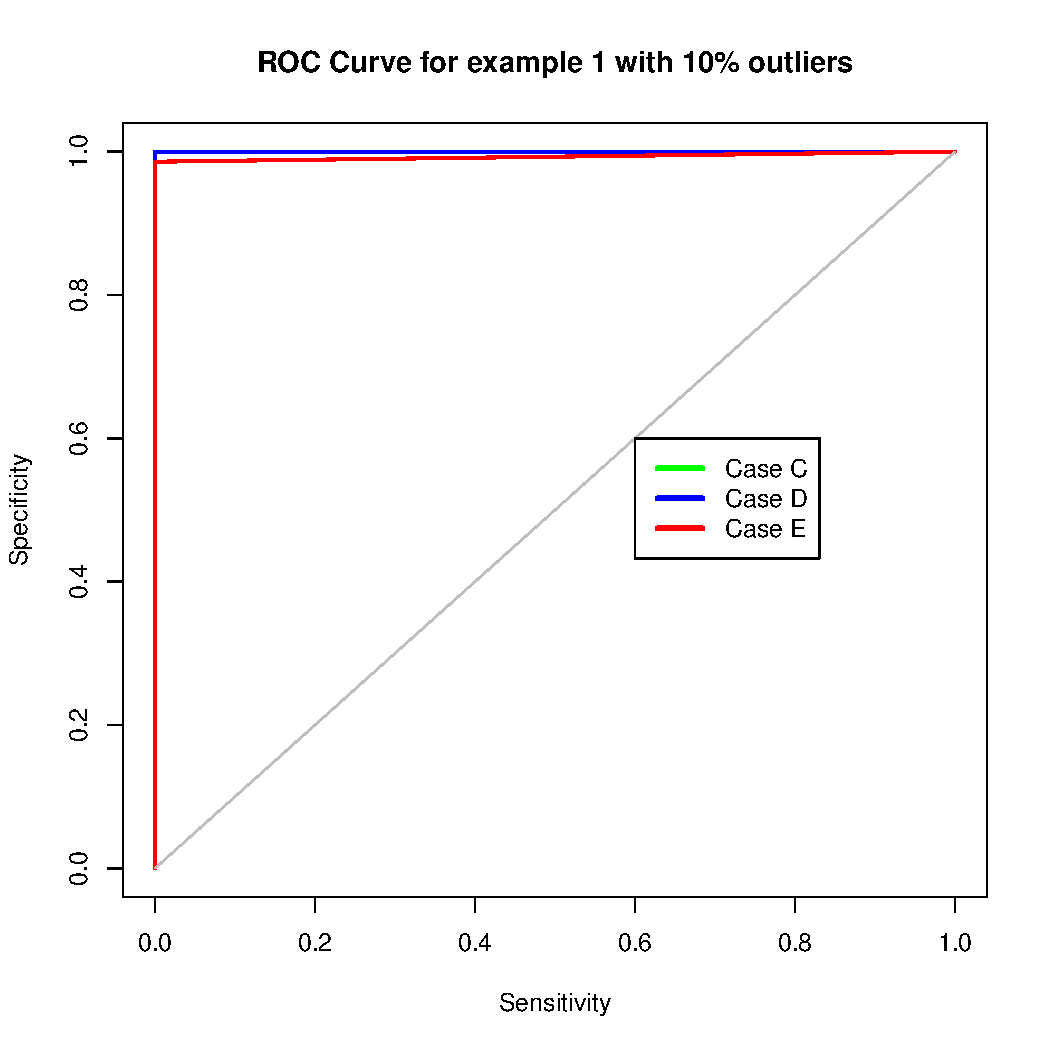
\includegraphics[width=\maxwidth]{figure/unnamed-chunk-2-1} 

\end{knitrout}
% ----------------------------- ROC Curve for example 1 with 20% outliers-------------------------------%
\begin{knitrout}
\definecolor{shadecolor}{rgb}{0.969, 0.969, 0.969}\color{fgcolor}
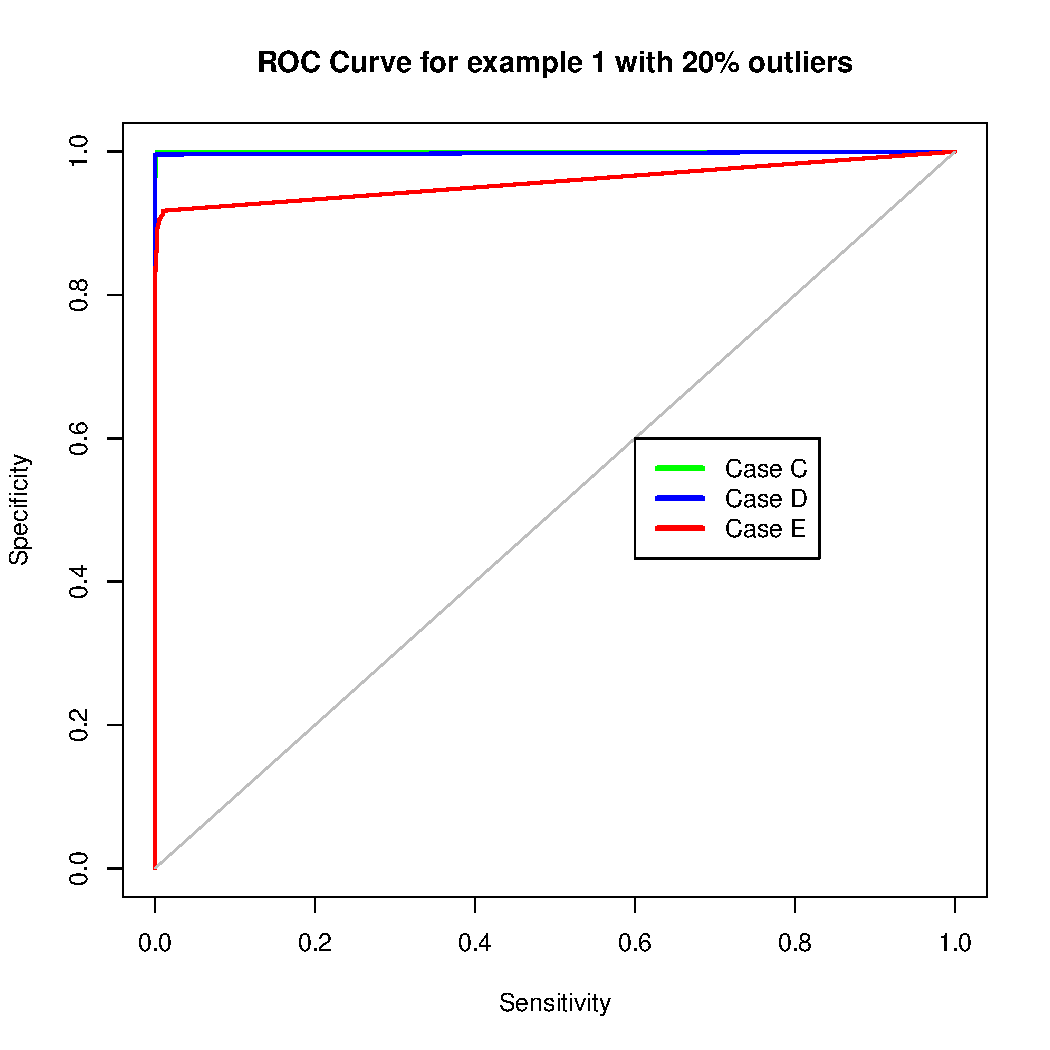
\includegraphics[width=\maxwidth]{figure/unnamed-chunk-3-1} 

\end{knitrout}
% ----------------------------- ROC Curve for example 1 with 30% outliers-------------------------------%
\begin{knitrout}
\definecolor{shadecolor}{rgb}{0.969, 0.969, 0.969}\color{fgcolor}
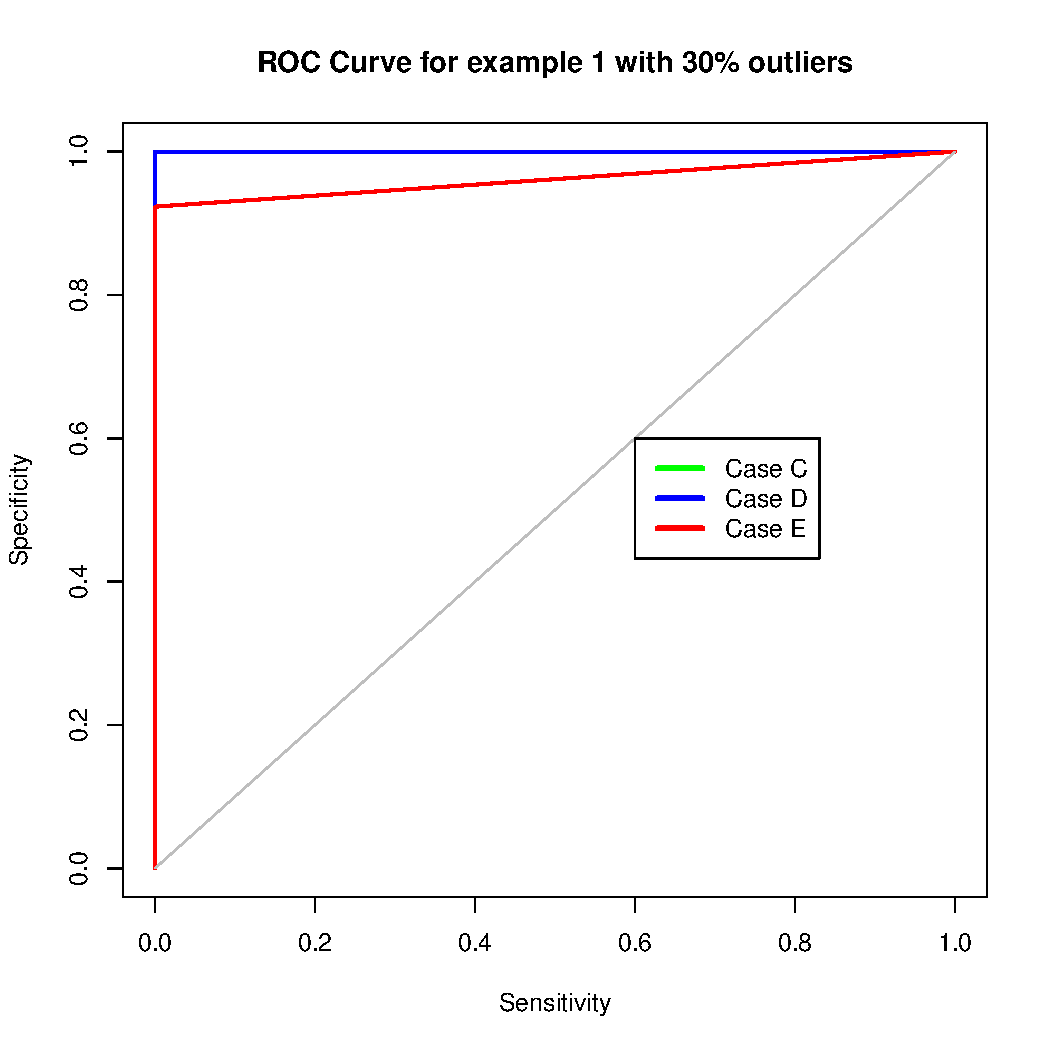
\includegraphics[width=\maxwidth]{figure/unnamed-chunk-4-1} 

\end{knitrout}

% ----------------------------- ROC Curve for example 2 with 10% outliers-------------------------------%
\begin{knitrout}
\definecolor{shadecolor}{rgb}{0.969, 0.969, 0.969}\color{fgcolor}
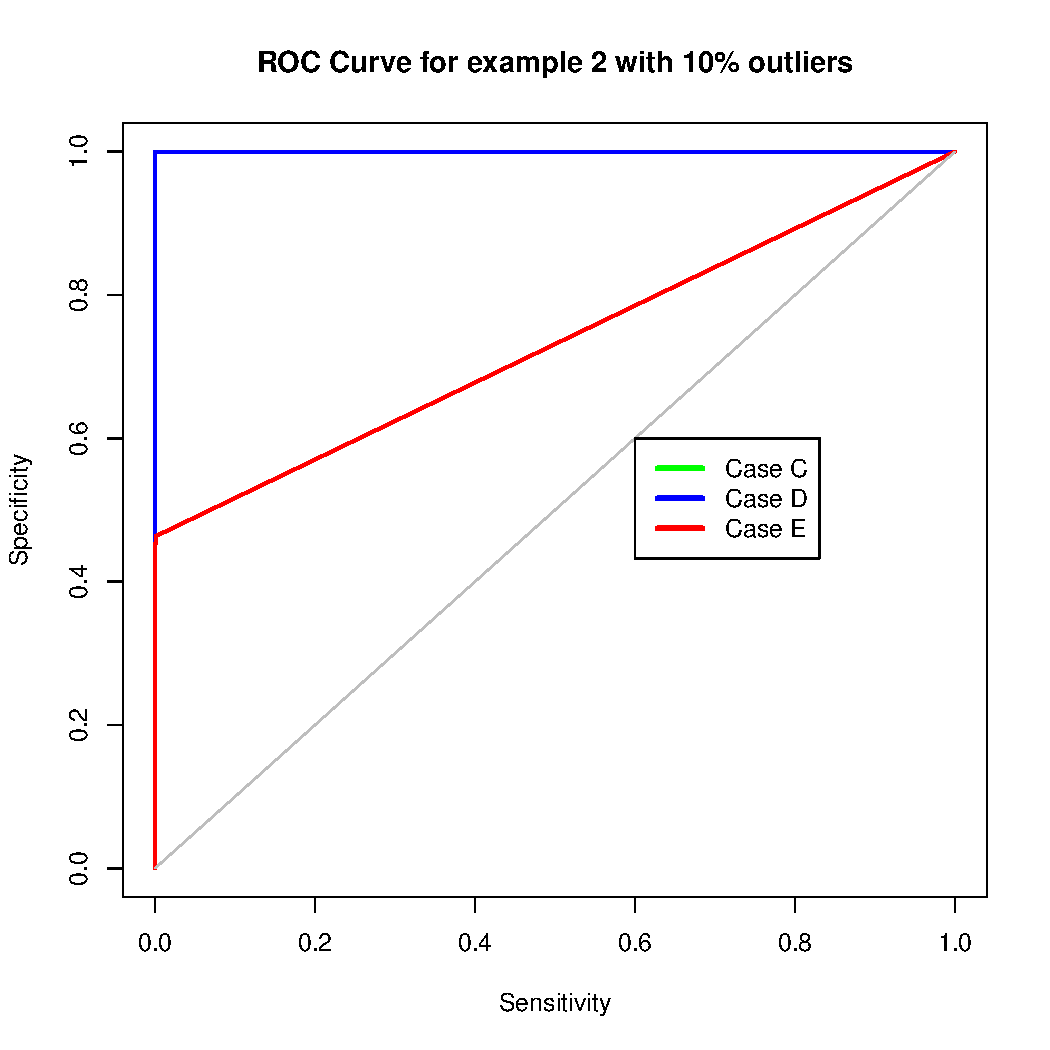
\includegraphics[width=\maxwidth]{figure/unnamed-chunk-5-1} 

\end{knitrout}

% ----------------------------- ROC Curve for example 2 with 20% outliers-------------------------------%
\begin{knitrout}
\definecolor{shadecolor}{rgb}{0.969, 0.969, 0.969}\color{fgcolor}
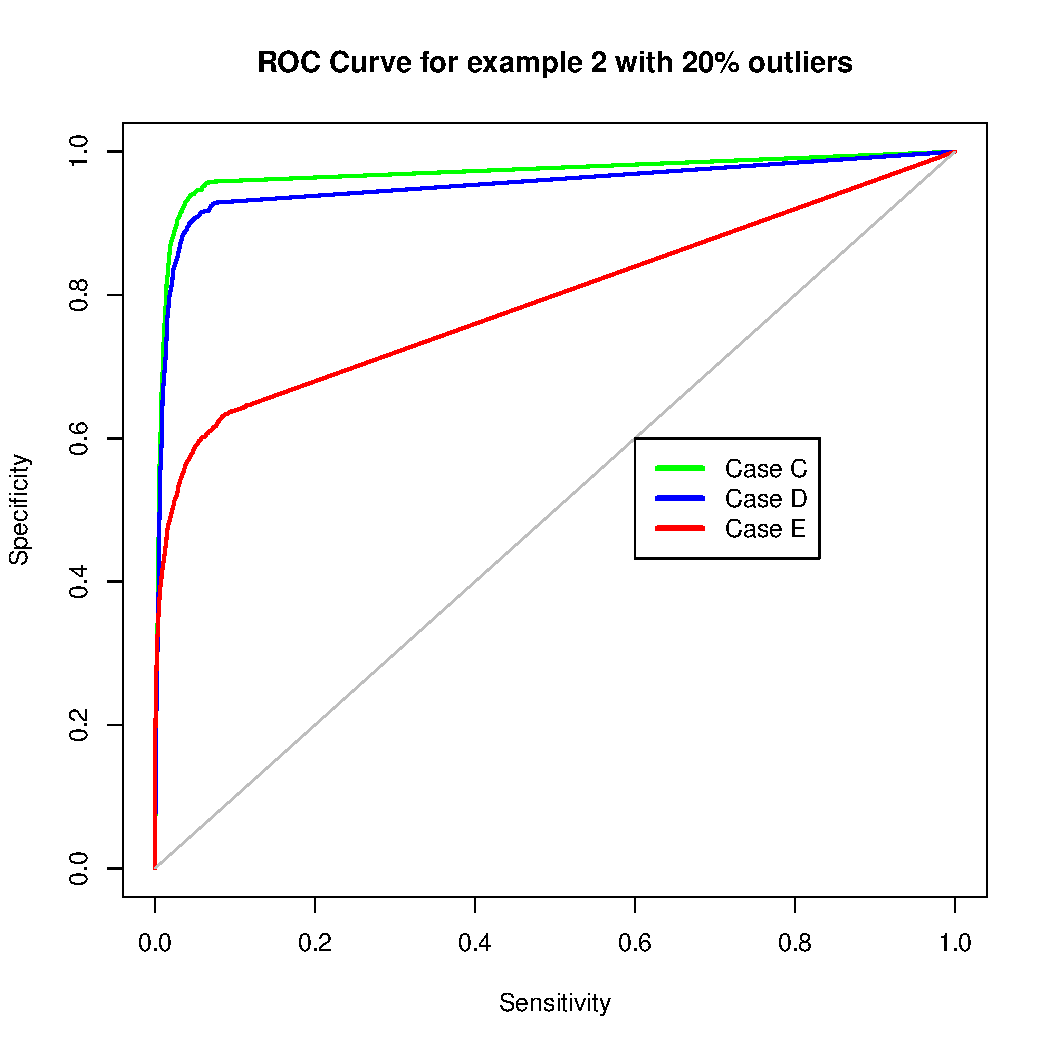
\includegraphics[width=\maxwidth]{figure/unnamed-chunk-6-1} 

\end{knitrout}

% ----------------------------- ROC Curve for example 2 with 30% outliers-------------------------------%
\begin{knitrout}
\definecolor{shadecolor}{rgb}{0.969, 0.969, 0.969}\color{fgcolor}
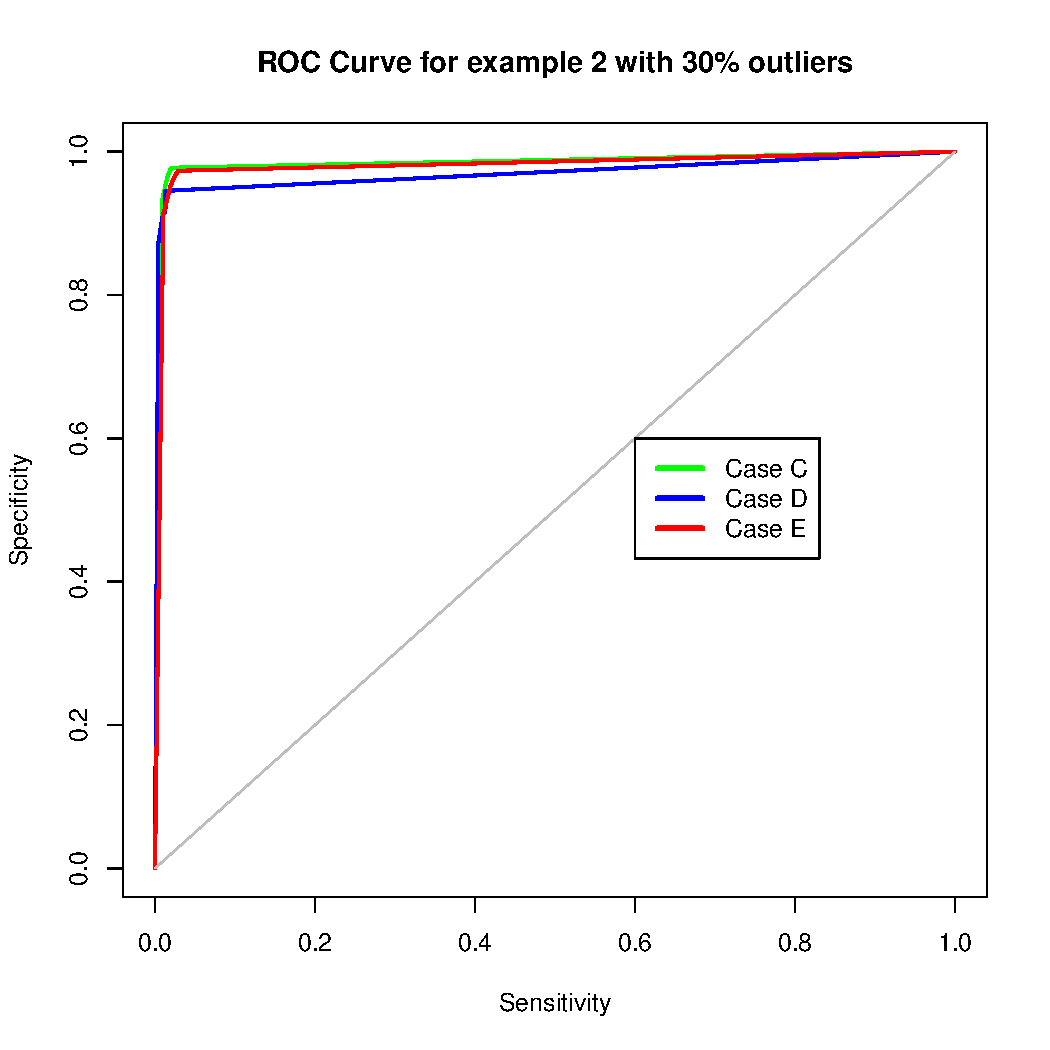
\includegraphics[width=\maxwidth]{figure/unnamed-chunk-7-1} 

\end{knitrout}
\end{document}
